
\documentclass[conference]{IEEEtran}

\usepackage{blindtext, graphicx}
\usepackage{float}
\usepackage{caption}
\usepackage{authblk}



\begin{document}

\title{Data Acquisition and Hardware Setup Development for Implementation of Feedback Control and Obstacle Detection for Car Type Robot}


\author{Akshay A. Dhotre}
 
\affil{Department of Electronics Engineering \\ 
Walchand College of Engineering, Sangli \\ Email: a2dhotre@gmail.com}


\author{Dr. Mrs. S. S. Deshpande}
\affil{Professor, Walchand College of Engineering, Sangli \\ Email: shraddha.deshpande@walchandsangli.ac.in}
 
\author{Dr. Mrs. R. A. Walambe}
\affil{Research Fellow, PVG's COET, Pune \\ Email: rahee.walambe@gmail.com}


\author{Dr. Mrs. V.A. Joshi}
\affil{Professor, PVG's COET, Pune \\ Email: amarvru@yahoo.co.in}



\renewcommand\Authands{ and }

% make the title area
\maketitle


\begin{abstract}
%\boldmath
	Auto-navigation is an essential feature in development of autonomous robots.
	This paper describes a hardware setup to implement feedback control and obstacle detection for car type robot. The motion planner developed in \cite{paper1} \cite{paper2} provides the reference states. The feedback algorithm which is currently under development uses the physical sensory data and compares it with these reference values to find and correct the actual states of the vehicle. The feedback algorithm is being developed to track the motion planner. The implementation is based on Raspberry Pi (RPi) board. 
	This board reads physical data from sensors and processes it, our focus in this paper is the development of the hardware setup for implementation of the feedback control and obstacle detection algorithms.
\end{abstract}
% IEEEtran.cls defaults to using nonbold math in the Abstract.


% Note that keywords are not normally used for peerreview papers.
\begin{IEEEkeywords}
Raspberry Pi, Light Detection and Ranging (LIDAR), Magnetometer, Rotary Encoder, Pulse Width Modulation (PWM), General purpose input-output (gpio).
\end{IEEEkeywords}


\IEEEpeerreviewmaketitle




\section{Introduction}
The vision of self-driving and parking cars promises to bring fundamental change to one of the most essential aspects of our daily lives. 
Although automatic gears are common in cars, complete auto-drive car is still not a reality. 
Autonomous driving involves high machine intelligence and decision making capabilities for the vehicle.
In [1], we have presented the Differential Flatness Based Nonholonomic Motion Planner for a Car type Mobile Robot. In [2] we have shown how the spline based optimization can be incorporated in this motion planner to avoid the singularities and generate the shortest path which also satisfy the nonholonomic and curvature constraints. However, the development discussed in both [1] and [2] uses the open loop control and hence there are certain issues in generating the exact trajectories on the hardware platform. These issues are highlighted in [2]. The way forward is to implement the feedback control algorithm which compares the expected states from motion planner with the actual states obtained from the sensors. The error is then processed using the nonlinear feedback controller such as [4] and \cite{paper45}.  Corrected control inputs are generated which will force the car to follow the path generated by the motion planner accurately. 

This paper discusses the hardware setup developed for implementing the two essential algorithms viz; Feedback Control and Obstacle Detection. The Feedback Control requires the accurate knowledge of the states of the car (i.e.position in moving plane and orientation angle). These can be obtained from the sensors mounted on the vehicle. In our case, the three sensors which are under consideration and which generates the four car states are: Magnetometer(orientation angle-$ \theta $), Potentiometer(Steering angle-$ \phi $) and Optical Encoder(position of car-x,y). Acquiring the accurate data which can be directly used in a feedback controller is of at most importance for accurate path tracking. The focus of this paper is on this data acquisition part of the implementation. Section 2 gives the system overview. We have discussed the hardware setup including the sensors and the SOC that is used for this development in section 3. 

The other aspect of work is the implementation of Obstacle Detection Algorithm. For the efficient collision avoidance in a static/dynamic environment, it is necessary that the obstacles are detected accurately. The LIDAR based OD algorithm [3] is currently under development. In section 4, we have discussed the hardware setup for the same followed by the results in section 5. Section 6 discusses the conclusion and future scope.  


\section{Overview of system}
System is based on R Pi board \cite{paper10}, which has quad core ARM processor, 1 GB of RAM and 40 GPIOS. It has support for open source operating systems and large community support.

Figure 1 shows the basic block diagram of system. Raspberry Pi will collect data from LIDAR (Light detection and ranging) module, compass magnetometer, rotary encoder and potentiometer on steering motor. 
LIDAR module will give distances from obstacles around which will be useful to plan path and avoid obstacles. 
Compass magnetometer will give orientation angle of vehicle. 
Rotary encoder will help to calculate distance traveled and speed. 
Steering angle can be detected using potentiometer fitted to steering servo motor.

\begin{figure}[h]
\centering
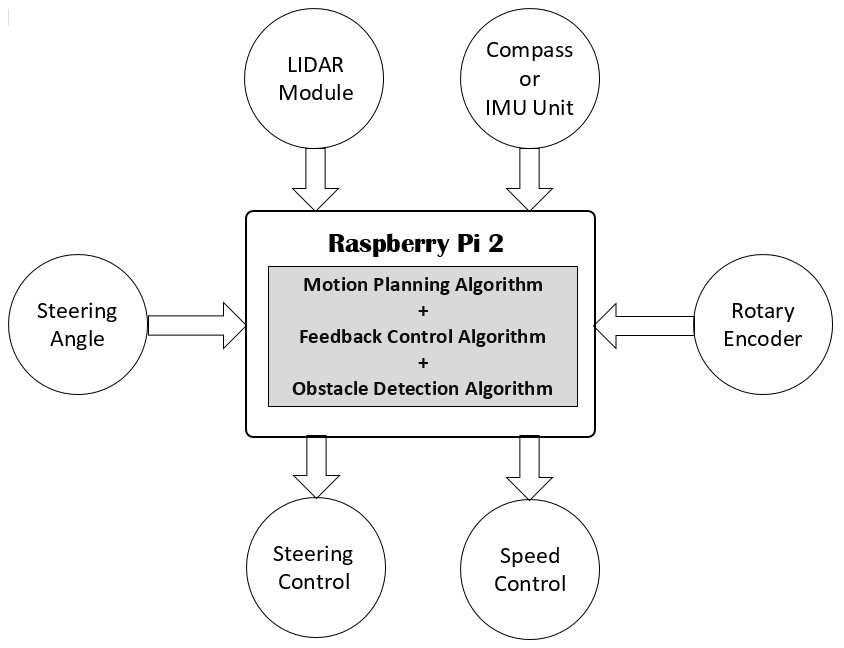
\includegraphics[width=1\linewidth]{block_diagram}
\caption{Block Diagram of System}
\end{figure}

\section{Data Acquisition for Feedback Control Algorithm}
Control algorithm mainly consists of motion planner algorithm \cite{paper1} \cite{paper2}, which decides the motion of robot according to inputs. Inputs can be co-ordinates starting point and end point on plane of motion. Main part of feedback control is to read data from sensors and producing PWM signals.
\subsection{Interfacing Magnetometer to RPi}



\begin{figure}[H]
	\centering
	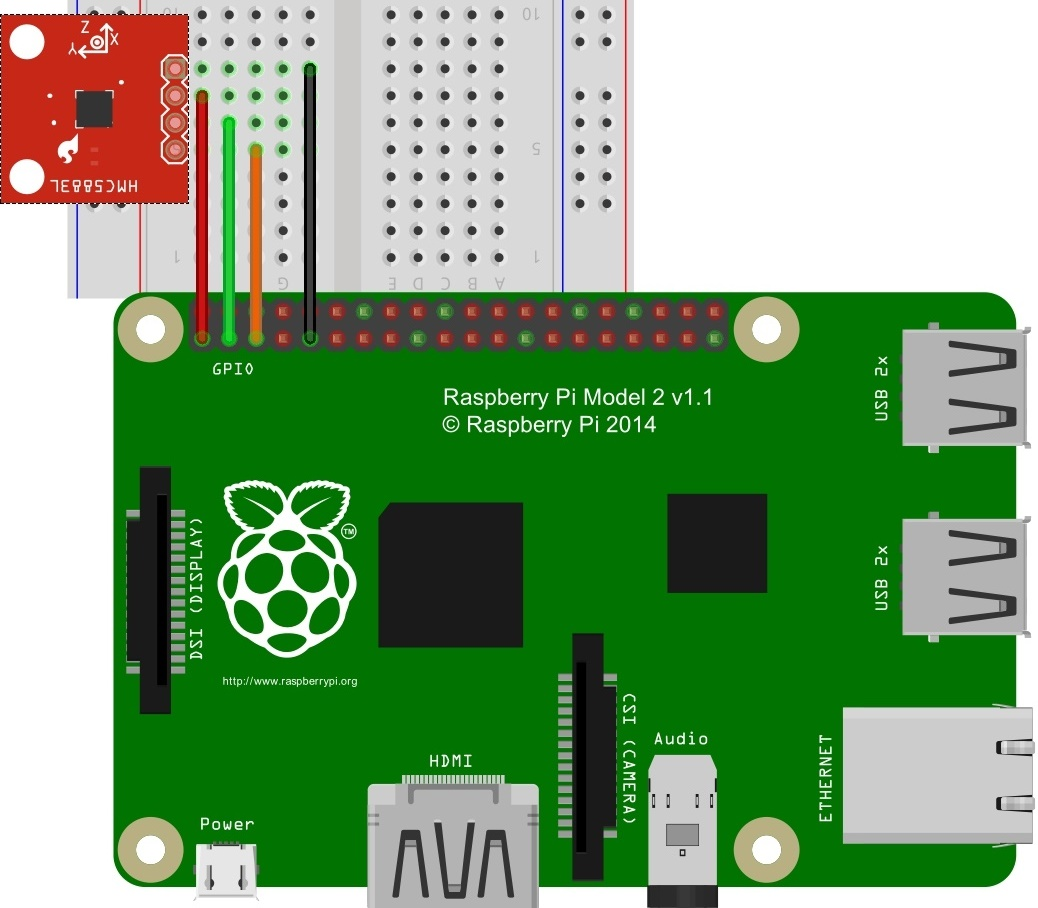
\includegraphics[width=0.7\linewidth]{rpi_mag}
	\caption{Magnetometer Connected to RPi}
	\label{fig:rpi_mag}
\end{figure}

Magnetometer module measures the earths magnetic field in three axes. It provides individual readings for each axis, which may be used separately or together for 3D calculations. Also it can measure raw magnetic strength of nearby magnetic source.

Here HCM5883L module is used to find orientation angle of vehicle. This module communicates with R Pi using I2C bus. Figure 2 shows the connection between RPi and magnetometer.

\subsection{Interfacing Encoder to RPi}

Encoders are often used in intelligent machines to control their movements. In case of car type robots rotary optical encoders are used to find distance traveled by it, so as to find its relative position. Also using encoder readings we can calculate speed of robot. Figure 3 shows encoder interfaced to R Pi through gpios. The encoder used for the car model is from Jencoder \cite{paper9}. The ppr rating of encoder is 2000 and it can be operated using 5V to 24V DC supply voltage.

\begin{figure}[H]
	\centering
	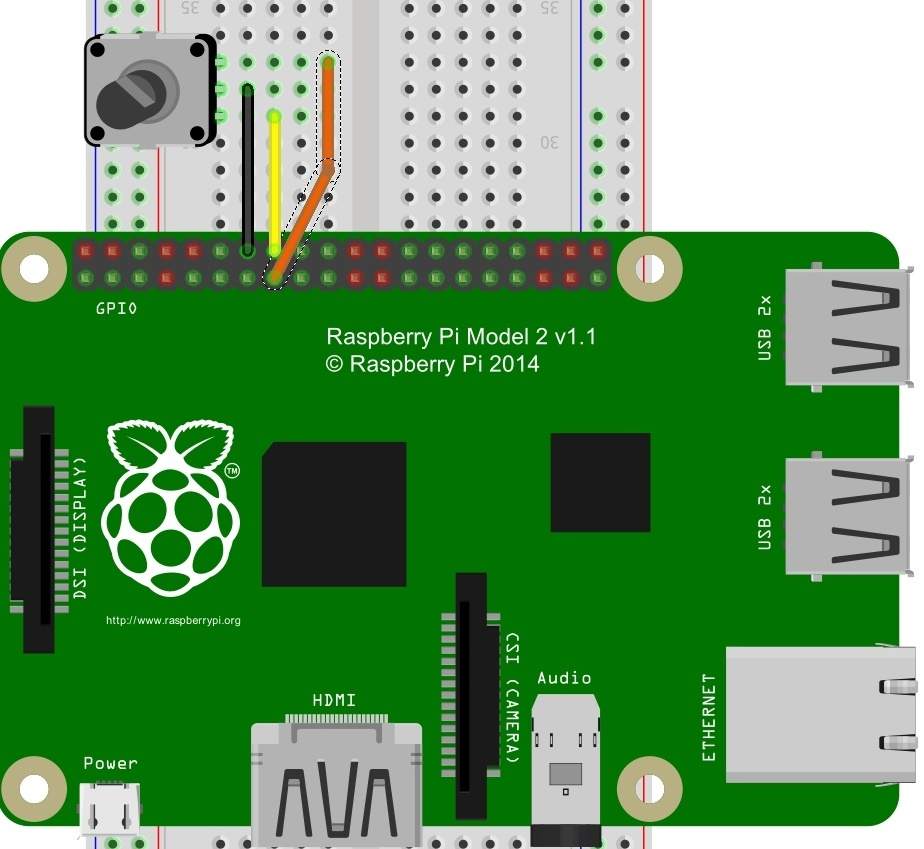
\includegraphics[width=0.7\linewidth]{rpi_encoder_connection}
	\caption{RPi and Encoder Connection}
	\label{fig:rpi_encoder_connection}
\end{figure}


\subsection{Interfacing Potentiometer to RPi}

\begin{figure}[H]
	\centering
	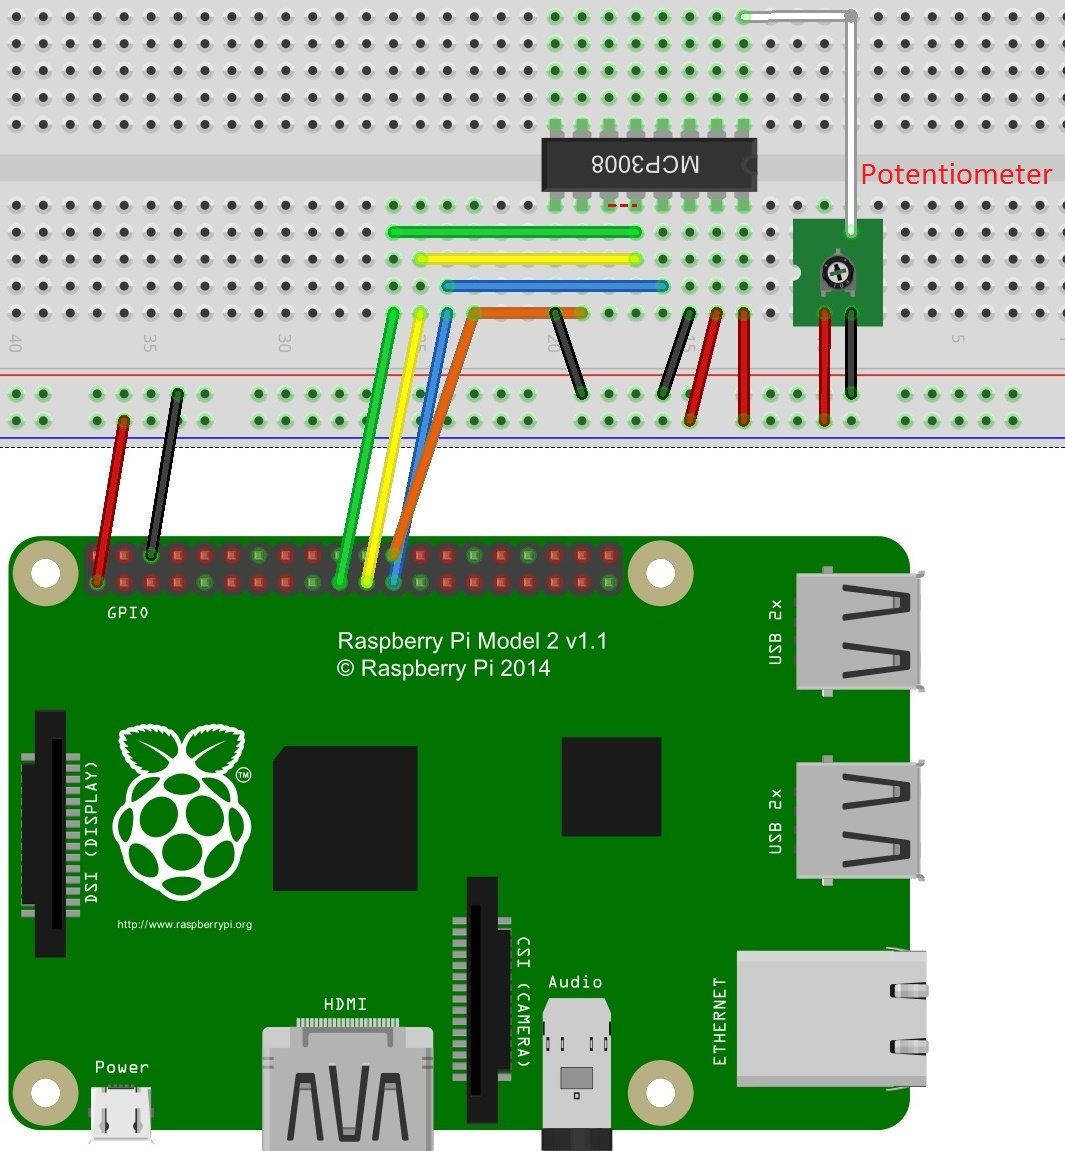
\includegraphics[width=0.7\linewidth]{rpi_mcp}
	\caption{Potentiometer connected to R Pi via ADC}
	\label{fig:rpi_mcp}
\end{figure}

Besides having 40 gpios, Raspberry Pi 2 has one downside. It has no analog supporting pin.
So, to measure analog voltages required in some applications is not directly possible.
Here we have to use Analog to digital converter to read voltage from potentiometer.

Figure 4 shows the potentiometer connected to ADC IC and connection to RPi. MCP3008 is 8-Channel ADC used which gives capability to read analog values. This IC communicates using SPI (Serial Peripheral Interface) bus. \cite{paper7}

\subsection{Generating PWM from RPi}
Raspberry pi has 40 gpio pins, one of which has hardware PWM support (Pin number 12). 
There are many libraries written for it which support software PWM on other gpio pins. 
They can be useful for applications requiring more number of motor controls or LED controls.
WiringPi is one of the popular library in R Pi which has function to generate software PWM on any number of GPIO pins.\cite{paper6}

``int softPwmCreate (int pin, int initValue, int Range) ;"

This creates softwre controlled PWM pin. If we give Range as 100 and initial value 0, we can genertae PWM with width anything from 0 to 100.

``void softPwmWrite (int pin, int value) ;"

This gives the value to the pin, to create required pulse width.

The PWM signals generated in this system are using this technique.

\subsection{Feedback Control Algorithm}

\begin{figure}[H]
	\centering
	\includegraphics[width=0.3\linewidth]{Flow_chart}
	\caption{Feedback Control Flow Chart}
\end{figure}

Figure 5 shows the flow chart which describes feedback control operation. This algorithm calculates control signal values in form of structures to travel from starting point to end point. 
Initially the values are taken as default i.e. first value calculated by motion planner. While car starts motion, data from sensors is collected, viz. steering angle from potentiometer, orientation angle from magnetometer and distance travellded from encoder. This data is collected in structures and then compared to initially calculated values by motion planner. Then the control signals in form of PWM are so generated that the error between calculated parameters and parameters obtained from sensors is minimum as possible.\cite{paper4}

\section{Data Acquisition for Obstacle Detection}
For autonomous driving car the detection of static or moving obstacle is essential to ensure safety. 
To implement such obstacle detection feature there are various methods like use of Infra-Red light based detectors, use of camera, using LIDAR etc. 
Here obstacle detection is done using LIDAR based Sensor.\cite{paper5}

\begin{figure}[H]
	\centering
	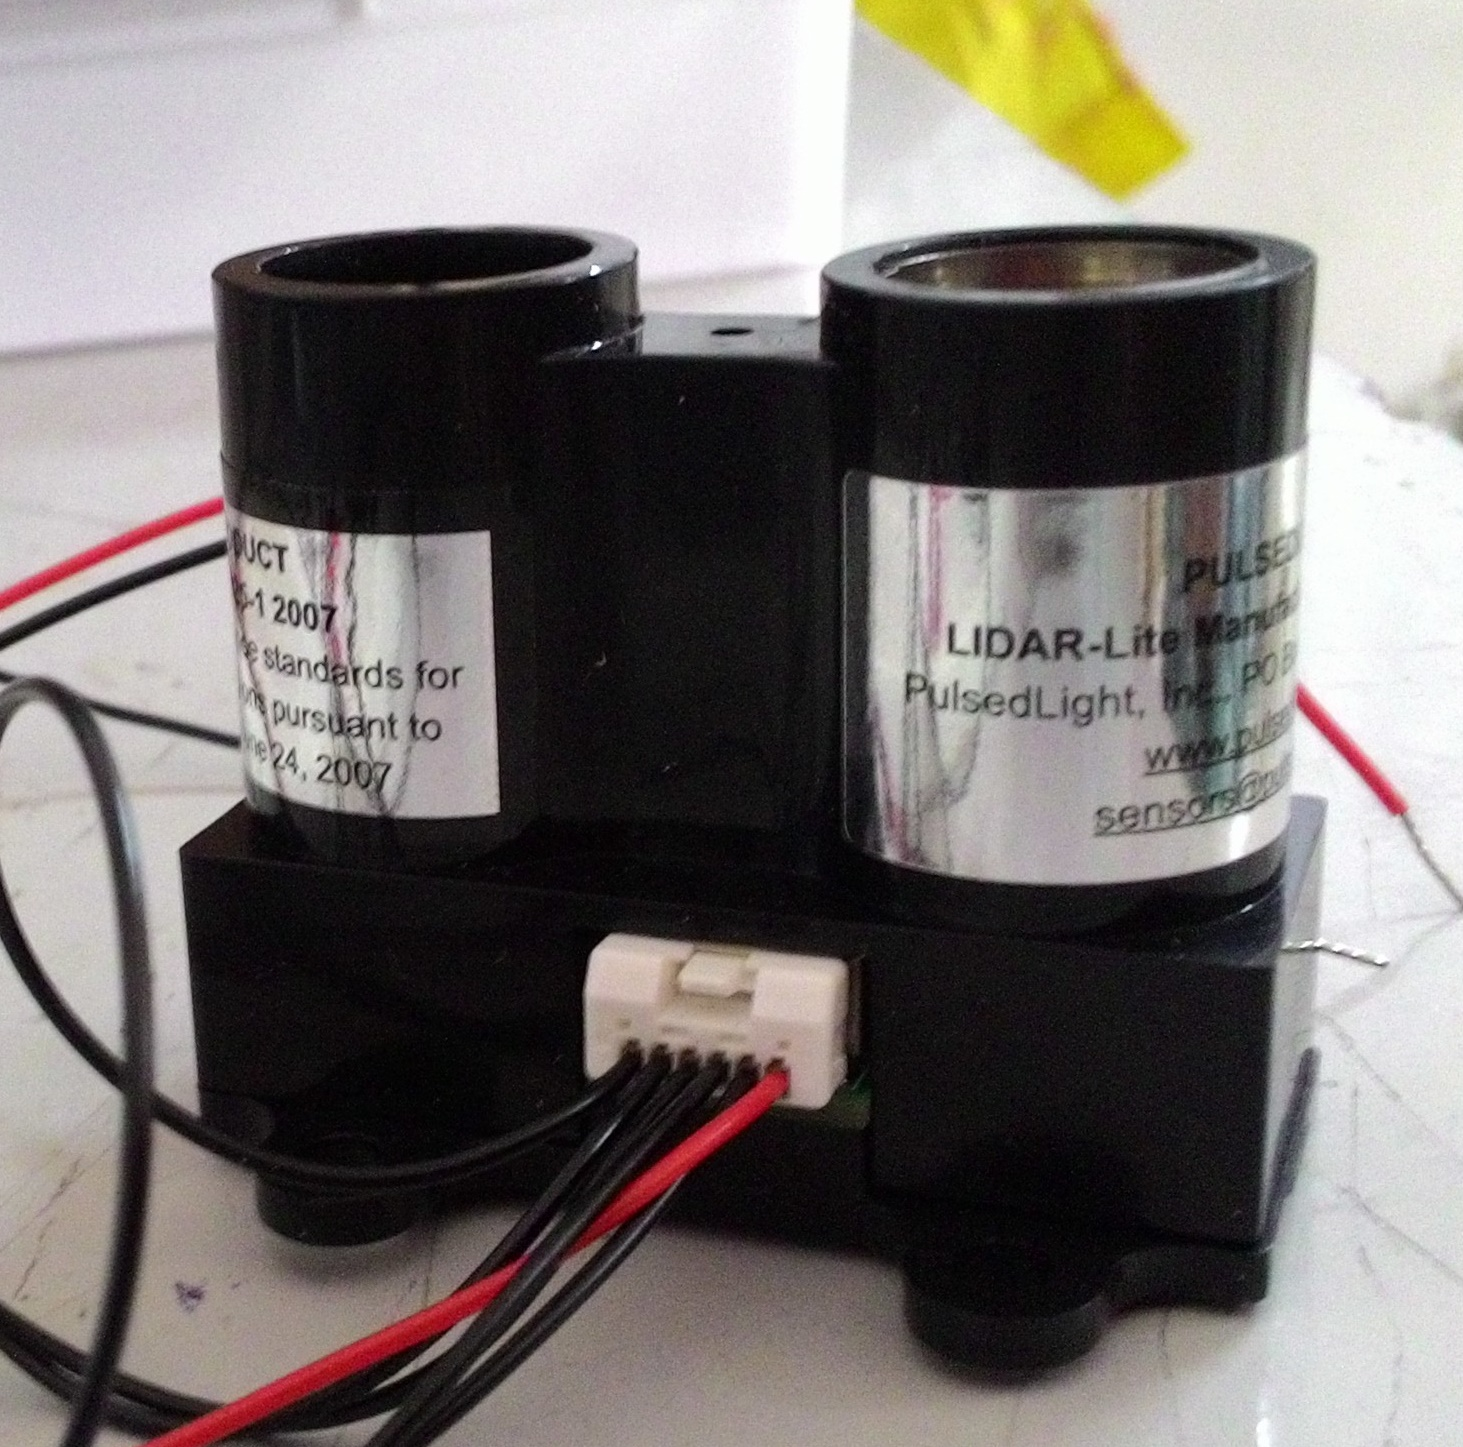
\includegraphics[width=0.4\linewidth]{lidar}
	\caption{PulsedLight Lidar Module}
	\label{fig:lidar}
\end{figure}

LIDAR is a remote sensing method that uses light in the form of a pulsed laser to measure ranges (variable distances) to the earth. These light pulses combined with other data recorded by the airborne system generate precise, three-dimensional information about the shape of the Earth and its surface characteristics. LIDAR based sensor gives distances of obstacles nearby, so that we can use them to interpret environment around robot.\cite{paper3} For using with RPi, PulsedLight LIDAR module (shown in figure 6) is useful which communicates to RPi using I2C protocol.  

This module gives direct distance of obstacle in front of it. So, to know about obstacles around robot, we can rotate module and get data for 180 degree around or for 360 degree around. We have mounted the LIDAR on servo motor as shown in Fig 7 and we measure the distance of LIDAR from its surrounding objects by rotating the servo motor. We get the distance reading in mm at every 1 degree rotation. The reading is the distance at which the laser beam is obstructed.  By predetermined the safety perimeter ( e.g. 10cm), we can detect the objects inside that perimeter and accordingly plan our path so as to avoid them. 

\begin{figure}[H]
\centering
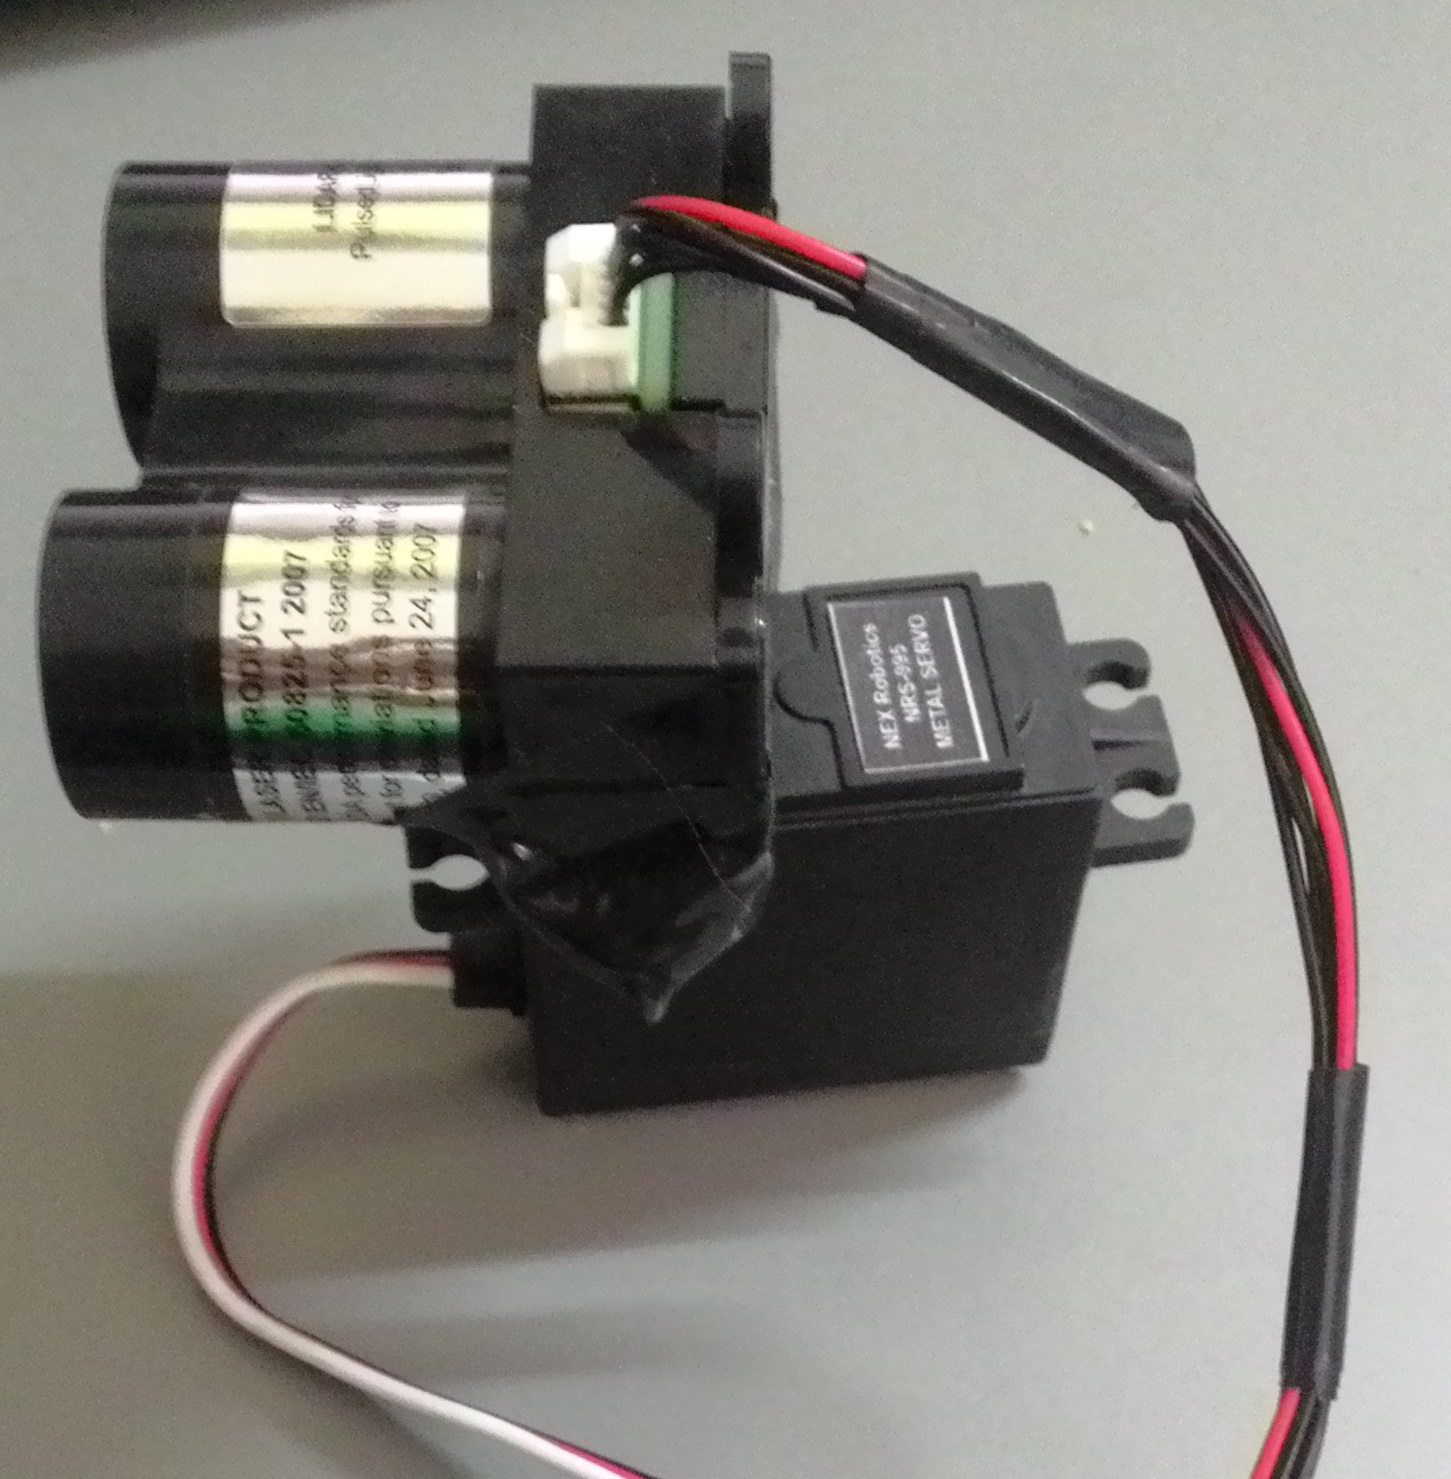
\includegraphics[width=0.4\linewidth]{lidar_servo}
\caption{LIDAR Module Mounted on Servo Motor}
\label{fig:lidar_servo}
\end{figure}

For this setup, we can precisely control the angle of servo motor, and collect data of obstacle distance corresponding to angle. Then this data is communicated to motion planner so that it avoids the angles which have obstacle nearby. 

\section{Results}

\subsection{Magnetometer Data}
 Magnetometer gives readings for x, y and z directions. Using these values we can calculate orientation angle.
 
 Formula used to calculate orientation angle is using inverse tangent function.
 
 \begin{center}
 	$ angle = [atan(\frac{x}{y})*360] /pi $
 \end{center}
 
 
 As car has movement is in x-y plane, no need to consider z axis value produced by magnetometer. Figure 8 shows output generated by magnetometer. 
 
\begin{figure}[H]
\centering
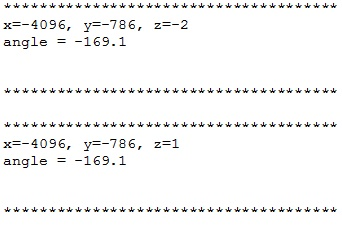
\includegraphics[width=0.9\linewidth]{magneto}
\caption{Screen-shot of Magnetometer Program Output}
\end{figure}

\subsection{Encoder Data}
Rotary encoder generates two pulse trains as it rotates. Using these two pulse trains the distance and direction (i.e. forward or reverse) can be found out. Also using distance traveled we can calculate speed of robot. Every encoder has its ppr value which means pulses per revolution. Using this value we can calculate distance traveled.

Formula for calculating distance traveled is: 

$ distance = (count * pi * diameter) / ppr $

here diameter is diameter of wheel attached t shaft of encoder. Figure 9 shows data produced by encoder on terminal window, when its code is runnning.

\begin{figure}[H]
\centering
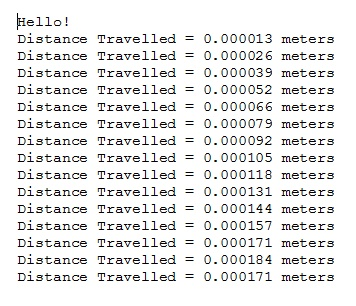
\includegraphics[width=0.9\linewidth]{enc}
\caption{Screen shot of Distance Measurement Program Output}
\end{figure}


\subsection{Potentiometer Data}
Potentiometer is interfaced using 10 bit ADC and the voltage is calibrated in steering angle, therefore the output is in form of angle in degrees.

To measure voltage of potentiometer we need to multiply ADC count output by ADC reference voltage and divide it by resolution of adc.

$ voltage = (count * reference \, voltage) / 2^{10} $ 

Here 10 is used because MCP3008 is 10 bit adc.

Steering angle is calculated from voltage value by multiplying with coefficient obtained by calibrating angle and voltage physically. Figure 10 shows the output of potentiometer program, which gives voltage and steering angle.


\begin{figure}[H]
\centering
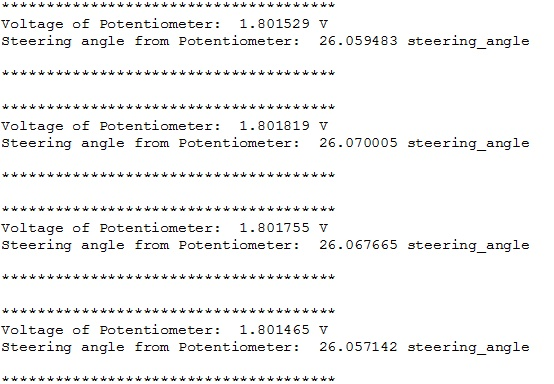
\includegraphics[width=1\linewidth]{pot}
\caption{Screen-shot of Steering Angle Measurement Program Output}
\end{figure}

\subsection{Robot Model after connecting all sensors}
Fugure 11 and 12 show the car model with all sensors except LIDAR module.\cite{paper11} 

\begin{figure}[H]
\centering
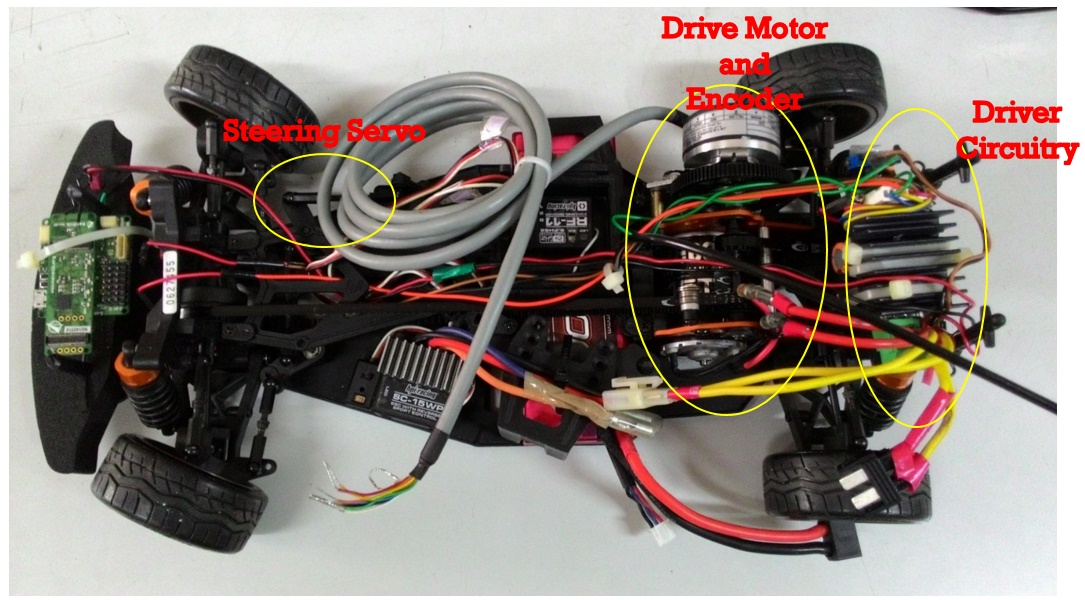
\includegraphics[width=0.8\linewidth]{car0}
\caption{Controls Present on Car Model}
\end{figure}


\begin{figure}[H]
\centering
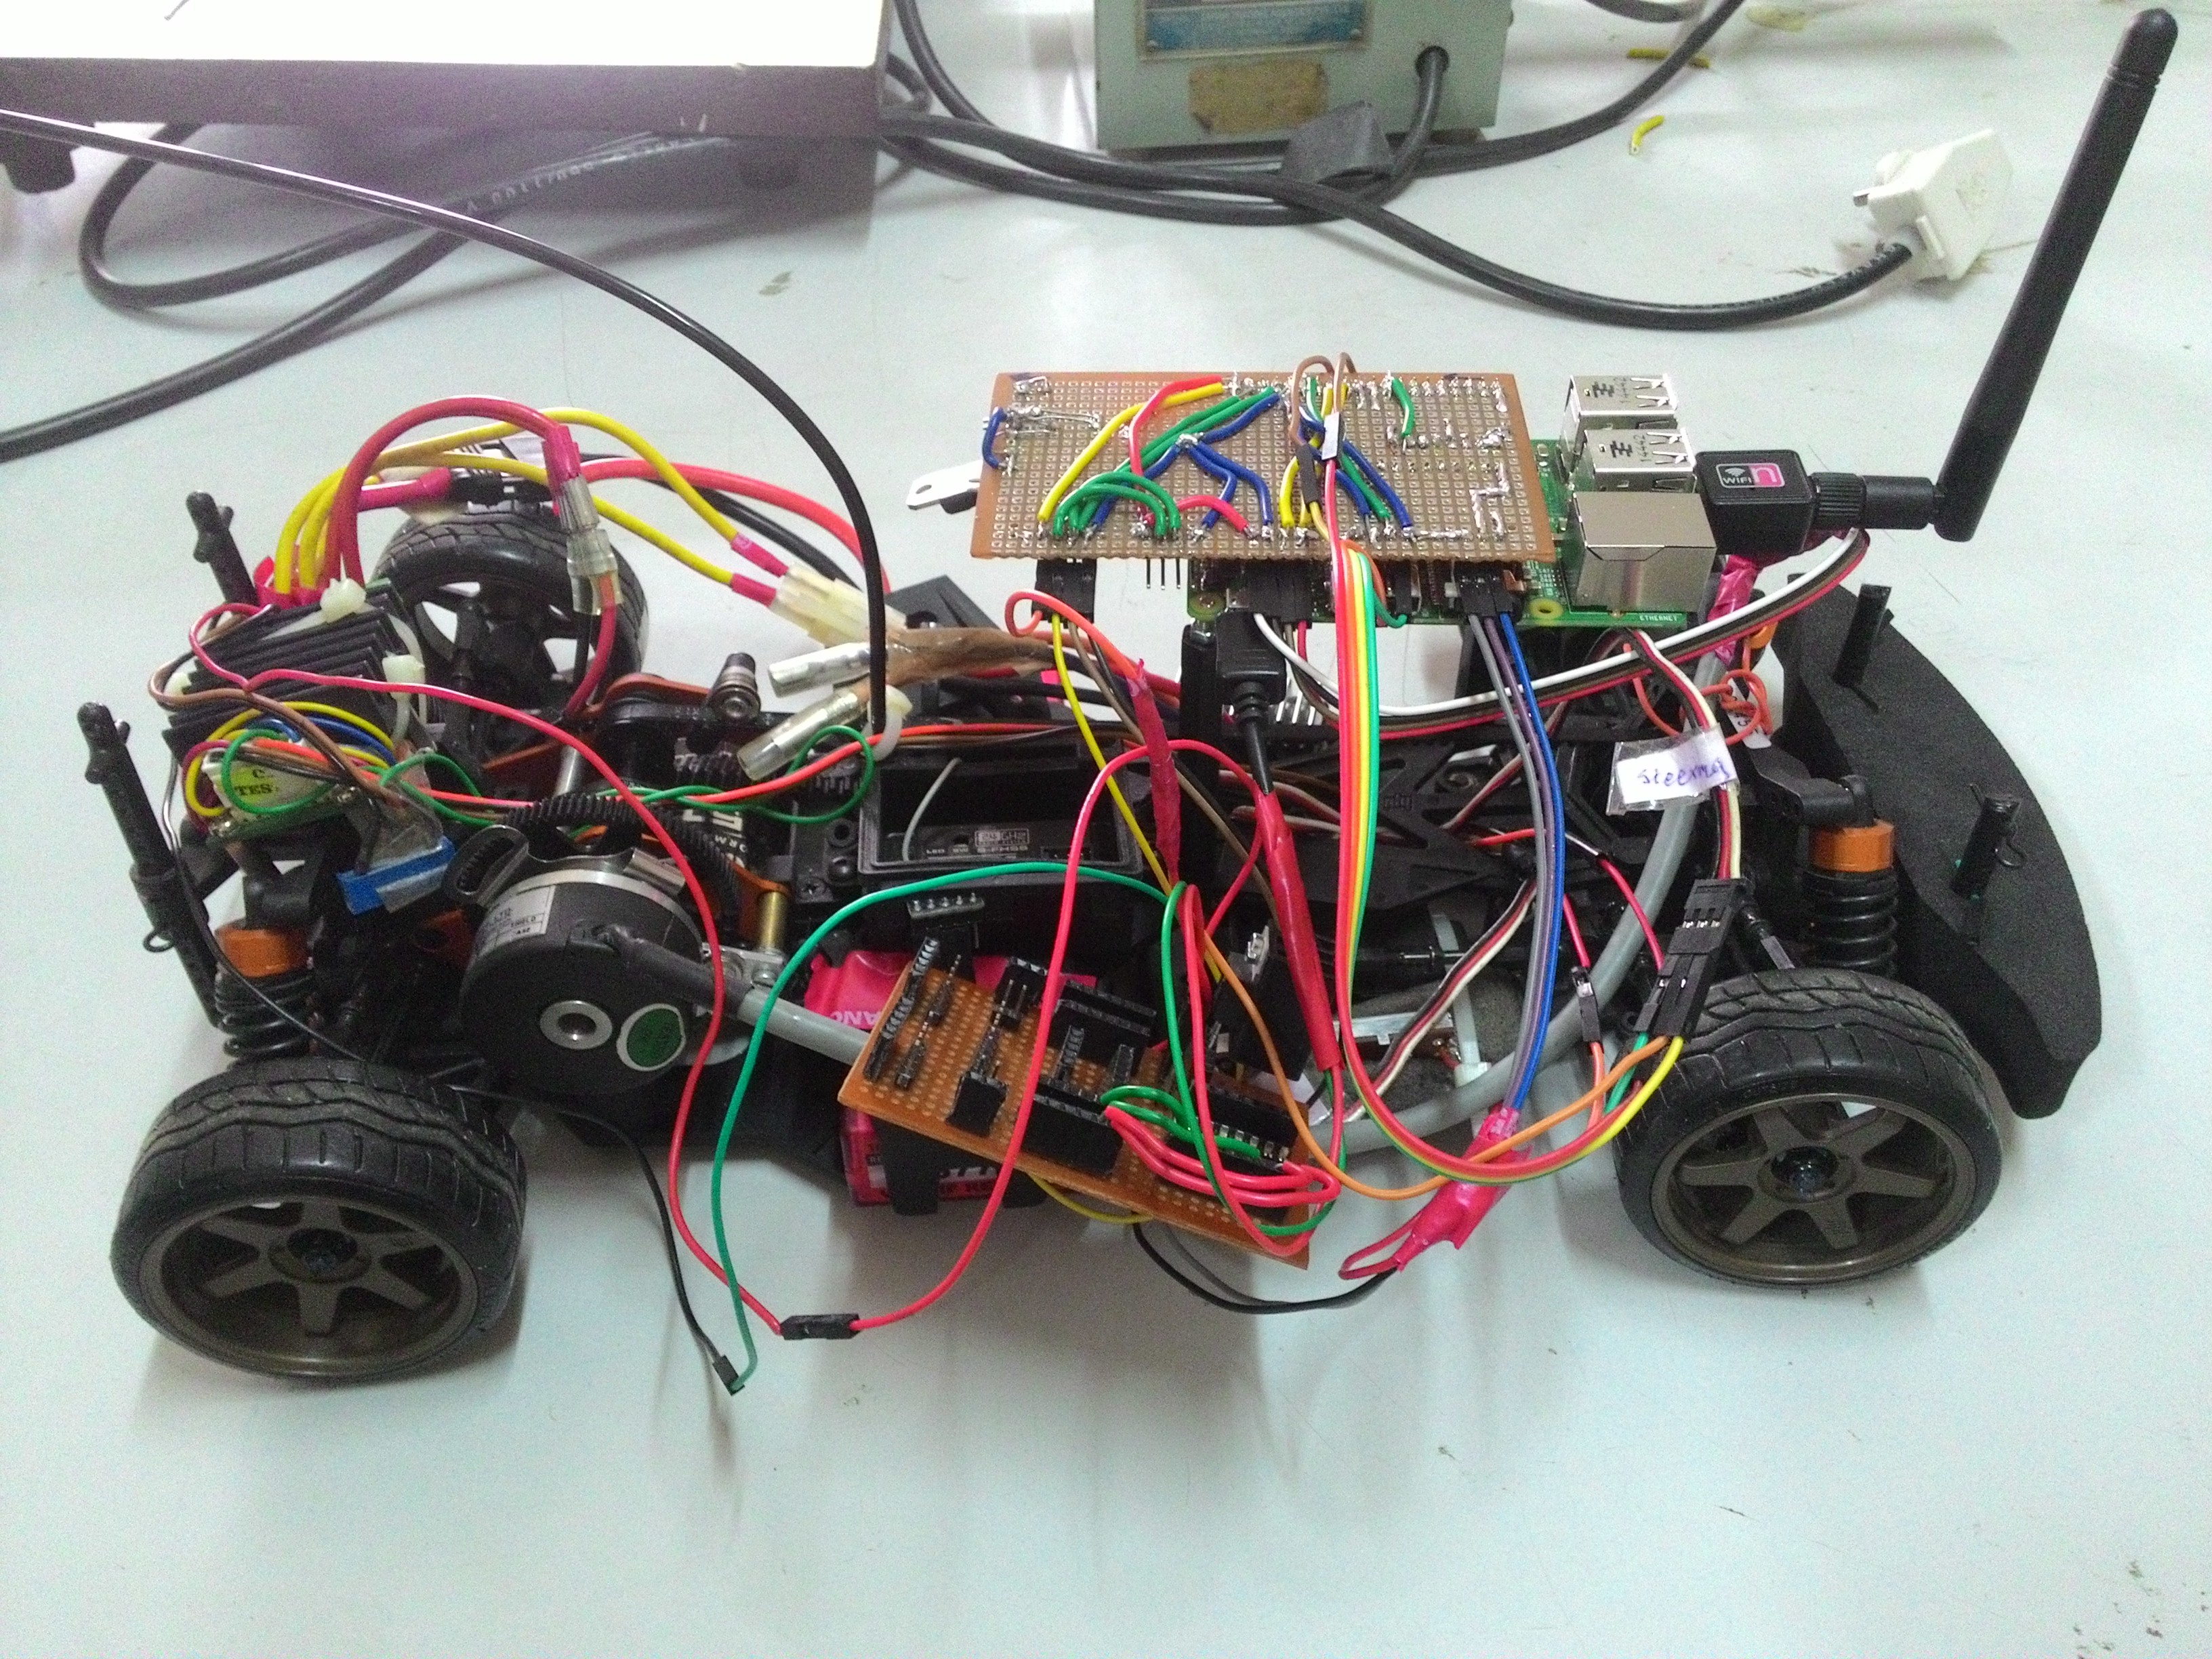
\includegraphics[width=0.8\linewidth]{car1}
\caption{Car Model with All Sensors Connected}
\end{figure}



% Can use something like this to put references on a page
% by themselves when using endfloat and the captionsoff option.
\ifCLASSOPTIONcaptionsoff
%  \newpage%
\fi

\section{ Conclusion and Future Scope}
 

The paper presented the development of hardware setup for the implementation of the Feedback Control algorithm and Obstacle Detection Algorithm. From the sensor data acquired using these setup consisting of the magnetometer, potentiometer and optical encoder, the feedback controller is currently being implemented. The LIDAR based obstacle detection algorithm is also under development. the obstacles will be marked on the map in run time and accordingly the path of the vehicle will be recalculated by the motion planner. 

\section{ ACKNOWLEDGEMENT} 

This project is funded under the WOS-A scheme (SR/ET/WOS-34/2013-14) of Dept of Science and Technology, Govt of India.

% references section

% can use a bibliography generated by BibTeX as a .bbl file
% BibTeX documentation can be easily obtained at:
% http://www.ctan.org/tex-archive/biblio/bibtex/contrib/doc/
% The IEEEtran BibTeX style support page is at:
% http://www.michaelshell.org/tex/ieeetran/bibtex/
%\bibliographystyle{IEEEtran}
% argument is your BibTeX string definitions and bibliography database(s)
%\bibliography{IEEEabrv,../bib/paper}
%
% <OR> manually copy in the resultant .bbl file
% set second argument of \begin to the number of references
% (used to reserve space for the reference number labels box)
\begin{thebibliography}{1}

\bibitem{paper1}
Agarwal N, Walambe R., Joshi V, Rao A. 'Integration of Grid Based Path Planning with a Differential Flatness Based Motion Planner in a Non-holonomic Car-type Mobile Robot' in Institution of Engineers Journal, November 2015, Pune, India 

\bibitem{paper2}
 Walambe R.A, Agarwal N. , Kale S. Joshi V. "Optimal Trajectory Generation for Car-Type Mobile Robot Using Spline Interpolation" in proceedings of ACODS 2016, Feb 2016, Trichy, India
 
 \bibitem{paper3}
 Jeffery Young, Milan Simic, `LIDAR and Monocular Based Overhanging Obstacle Detection', \textit{Knowledge-Based and Intelligent Information \& Engineering Systems 19th Annual Conference, KES-2015, Singapore}, Volume 60, 2015, Pages 1423–1432, September 2015.

 \bibitem{paper4}
 LU Jiangzhou, Sepanta Sakhavat, XIE Ming and Christian Laugier, `Sliding Mode Control for Nonholonomic Mobile Robot', \textit{In Proc. of the Int. Conf. on Control, Automation, Robotics and Vision, Singapore}, December 2000.
 
 \bibitem{paper45}
 A. De Luca, G. Oriolo and C. Samson,  `Feedback Control of a Nonholonomic Car-Like Robot', \textit{Lectures Notes in Control and Information Sciences 229}. Springer, ISBN 3-540-76219-1, 1998, 343p.
 
 \bibitem{paper5}
 PulsedLight, Makers of LIDAR-Lite: 500 Hz, Assignable I2C Addresses \& More, [Online] 2016,  http://pulsedlight3d.com (Accessed: 13 April 2016).
 
 \bibitem{paper6}
 Wiring Pi, [Online] 2016, http://wiringpi.com (Accessed: 13 April 2016).
 
 \bibitem{paper7}
 MCP3008 8-Channel 10-Bit A/D Converter, [Online] 2016, http://shaunsbennett.com/piblog/?p=266 (Accessed: 13 April 2016).
 
 \bibitem{paper8}
 James Brundell: HMC5883L magnetometer to Raspberry Pi connection notes, [Online] 2016, http://brundell.blogspot.in/2015/06/hmc5883l-magnetometer-to-raspberry-pi.html (Accessed: 13 April 2016).
 
 \bibitem{paper9}
 Jencoder,[Online] 2016, http://jencoder.com (Accessed: 13 April 2016).
 
 \bibitem{paper10}
 Raspberry Pi 2 Model B, [Online] 2016, https://www.raspberrypi.org/products/raspberry-pi-2-model-b (Accessed: 13 April 2016).
 
 \bibitem{paper11}
 762 RTR Sprint 2 Drift Sport,  [Online] 2016, http://hpiracing.world/en/kit/762
\end{thebibliography}

% biography section
% 
% If you have an EPS/PDF photo (graphicx package needed) extra braces are
% needed around the contents of the optional argument to biography to prevent
% the LaTeX parser from getting confused when it sees the complicated
% \includegraphics command within an optional argument. (You could create
% your own custom macro containing the \includegraphics command to make things
% simpler here.)
%\begin{biography}[{\includegraphics[width=1in,height=1.25in,clip,keepaspectratio]{mshell}}]{Michael Shell}
% or if you just want to reserve a space for a photo:

\begin{IEEEbiography}[{\includegraphics[width=1in,height=1.25in,clip,keepaspectratio]{picture}}]{John Doe}
\blindtext
\end{IEEEbiography}

% You can push biographies down or up by placing
% a \vfill before or after them. The appropriate
% use of \vfill depends on what kind of text is
% on the last page and whether or not the columns
% are being equalized.

%\vfill

% Can be used to pull up biographies so that the bottom of the last one
% is flush with the other column.
%\enlargethispage{-5in}




% that's all folks
\end{document}


